\documentclass[11pt]{report}

\usepackage[utf8]{inputenc}
\usepackage{xcolor}
\usepackage{filecontents}
\usepackage{tabularx}
\usepackage{csquotes}
\usepackage{hyperref}
\usepackage{parskip}
\usepackage{graphicx}
\usepackage{subcaption}
\usepackage{float}
\usepackage{paralist}

% Now also shows subsub section ect. in the table of contents
\setcounter{secnumdepth}{3}

% Create \fullref command
\newcommand*{\fullref}[1] {\hyperref[{#1}]{\ref*{#1} \nameref*{#1}}}

% Create a large quote that is centered
\newcommand*{\largequote}[1] {\begin{displayquote}\large \center "#1" \end{displayquote}}

% Change monospace font
\usepackage[T1]{fontenc}
\usepackage{inconsolata}

\usepackage[style=numeric, backend=biber]{biblatex}
\addbibresource{main.bib}

\title{Converting a monolithic application into a modular architecture}

\author{
  \parbox{.5\textwidth}{\centering
  Jessie Liauw A Fong \\
  \small \textbf{Student number}: 500726467 \\
  \small \textbf{Study}: Software Engineering \\
  \small \textbf{University}: Amsterdam University of Applied Sciences\\
}}

\begin{document}

\maketitle

\chapter{Preface}
I am Jessie Liauw A Fong, 20 years old. I was born in Amsterdam but moved to Zaandam and still live there. I started programming in 2010 when I was in the first class of middle school. After a year of programming my interest stagnated but in 2015 I chose to begin the study software engineering and I immediately felt that passion again and I haven’t lost that pasion since. In the end of 2015 I started my first software engineering job at The EsportsWall. This was a voluntary job because I did not have enough skills to get paid. 3 months later I did to start my internship at Endouble. I worked at Endouble for 1 year. 5 months as an intern and 7 months as an part time employee.

After I finished my internship at Endouble I started by own company JCB Development. Where I build high-end websites.

At the end of my time at Endouble I started a new parttime internship at Ximedes where I learned a lot about infrastructure. This is also the company I met my now co-worker Erik Schouten. He worked at CargoLedger and that is also where I work now. In the beginning of September 2018 I started a new company together with Stijn Claessen and Siebe Goos called EFFE Planning. This is also the company I will do my thesis in.

This thus means I know the ins and outs of the company.

\tableofcontents
\listoffigures

\chapter{Summary}

The company EFFE Planning makes employee schedule software. The business model of EFFE requires modules that are interchangeable. This is so EFFE can cater to bigger clients.
The question this research will answer is:

\largequote{What is the best way to transform a monolith into a modular architecture, where the modules are interchangeable with each other}

The first course of action was to order the quality attributes. These quality attributes were used to decide which modular architecture is the best fit for EFFE. This was the modular monolith architecture.

The backend framework used to implement the modular monolith is Django. Django is domain driven out of the box. In the frontend Vue was the framework that best aligned with the order of the quality attributes. The actual implementation that was used is Nuxt.js which is a framework on top of Vue. Nuxt.js was used because the current application already uses it.

When implementing the modular monolith there was a need to create an assembler and dissembler for the modules. This makes it easier for developers and in the deployment lane.


\chapter{Introduction}

\section{Motive}
EFFE as a company uses the SaaS model in order to comply to it’s expected growth. The basic SaaS model includes the basic application or MVP. This is in order to keep the application as abstract as possible. So that every company can connect their scheduling procedure to EFFE. But EFFE also wants to cater to the needs of bigger clients. This is why we created building blocks.

Building blocks are features that can be added/removed from the application. This can be done by the user or by EFFE. Examples of building blocks are white labeling, integration with frontend system and payroll integration. These building blocks are not required when acquiring EFFE but can be added one by one.

\section{Intention}
\label{sec:Intention}

So the question is how are we going to implement these building blocks. We have a few requirements:
\begin{itemize}
	\item They need to be interchangeable. Meaning the same building block can be changed with another one that does the same job with maybe extra functionality.
	
	\item They should be able to do everything programming related. From if else to database calls.
	
	\item They have impact on the frontend as well as the backend
	
	\item Building block should be completely separate from the application (loosely coupled)
\end{itemize}



\chapter{Research design}
This chapter contains the information on how the research will be conducted.

\section{Research objective}

\subsection{The problem}
\label{sec:TheProblem}

Right now EFFE is developing an application for employment agencies in which those employment agencies can schedule their employees automatically. The current application is really basic and there are requests from potential clients to implement certain features. We decided to add something to the business model called building blocks.

\largequote{Building blocks are interchangeable implementations of business logic that can be reused as efficient as possible}

EFFE is looking how to implement the building blocks in such a manner where scalability and maintainability are the focus.

\subsection{Objective}
The objective is to create a recommendation for an infrastructure on how to create and maintain that infrastructure. Where the focus lays on interchangeability and scalability of the different functionalities.

\begin{tabularx}{\linewidth}{|>{\hsize=.3\hsize}X|
		>{\hsize=.7\hsize}X|}
	\hline
	Stakeholder &
	Interest to the objective
	\\
	\hline
	EFFE &
	The obvious stakeholder is EFFE. EFFE will enhance its business model. But not only that. We will also create a better infrastructure which means that we can implement functionalities faster and cater more to the clients’ need.
	\\
	\hline
	Client &
	The client is also the one interested in this process. They are probably not interested into what happens behind the scenes but they are interested in the possibilities it adds for them to EFFE’s application
	\\
	\hline
\end{tabularx}

\section{Research framework}

\subsection{Objects}
This chapter describes who/what the objects are for this research and why.

\subsubsection{Backend architecture}
Arguably the most important object is the backend architecture. There is already a lot of research available regarding backend architecture. The backend is also the place where the business logic will be expressed. The backend connects to the database and thus needs a lot of attention when creating this section of the application.

\subsubsection{Frontend architecture}
The second object, frontend architecture, is a lesser known subject when looking at modularity of the actual system. Most of the big companies have a single frontend application per platform.

\subsubsection{Deployment lane}
\label{sec:DeploymentLane}
The backend and the frontend are the software side of the equation but the hardware is also important. Where does the software run? How does it run? The deployment lane is the section that pieces it all together. This object creates the hardware or virtual hardware. Sets this hardware up so it can then proceed to deploy the frontend and backend on the just created hardware. This process is very important and EFFE is not the first company wanting to adopt this. Which means there is already a lot of research in this area.

\subsubsection{Project manager}
\label{sec:ProjectManager}
The last object we want to research is the project manager. Because the research is focussed on implementing business logic in a modular way it is important to research what can go wrong when the business logic is translated to code.

\subsection{Research perspective}
The research perspective is straight forward. Because I am one of the founders of EFFE and I am also doing this research in name of EFFE it has my best interest to approach this research from the side of EFFE. This means that I will put more emphasis on sustainability than for example on the performance. Because for now performance can be dealt with later but if you want something to be sustainable you have to think about it from the ground up. Otherwise you will need to rewrite the whole architecture.

\subsection{Research sources}
This section will describe which sources will be used when evaluating the research objects. This will not include everything but a broad spectrum of the sources that may be used in the research:

\begin{itemize}
	\item \textbf{Modular architecture books: }In the end everything I need to know all comes down to modular programming. Modular programming is a very broad term and it is important to find how someone else may look at this term.
	
	\item \textbf{Implementations of modular programming: }Theory is one side of the coin. Everything can work perfectly in theory but when implementing the theoretic side you will find problems you haven't thought of before.
	
	\item \textbf{Critique from outside: }It is known that software architecture is an opinion based subject. This is because especially this area of software is fairly young. Software architecture did not have a lot of time to develop itself as far as some other aspects of software engineering such as operating systems. Because software architecture is young there are a lot of people voicing their opinions and it is important to look at the criticism on some of the architectures.
	
	\item \textbf{Researches on deployment of architecture: }I will be researching more than one architecture. Each architecture has its own development environment and deployment environment. The architecture of the servers on which the program runs is important but that will be heavily influenced by the architecture of the software. Nevertheless should it be researched separately from the software architecture
\end{itemize}

\subsection{Evaluation criteria}
These are the criteria or leading questions that will be asked to research objects. Note: not all evaluation criteria apply to all research objects:

\begin{itemize}
	\item \textbf{What is the biggest pitfall when implementing business logic: }As mentioned in \fullref{sec:ProjectManager} there will also be considered how business logic is translated to code. Because the building blocks will eventually be different based on business logic. The research will include what can go wrong in which way.
	
	\item \textbf{What are the most used architectures in this area: }There is always a reason why one architecture is very common and the other one isn't. In the research the reasoning will be extracted and reflected on.
	
	\item \textbf{What are the most upcoming architectures that are focused on modularity: }Again the whole research is based on the building blocks. These modular functionalities that can be designed via a common interface. Which architecture has which solution for this?
	
	\item \textbf{Which programming languages has the best attributes to complement the modularity: }Some languages are written purely for scripting or some are written to be focused on implementing algorithms more easily. Each programming language has its attributes and which of these attributes are most defining and important to a modular system.
	
	\item \textbf{Which quality attributes are deemed most important to EFFE?: }The quality attributes from ISO 205010 \cite{iso25010} are the backbone of an the architecture. In the research will describe which are most important to EFFE. It is then important to reflect the quality attributes we chose on the architectures.
\end{itemize}

\subsection{Research framework}

\begin{figure}[H]
	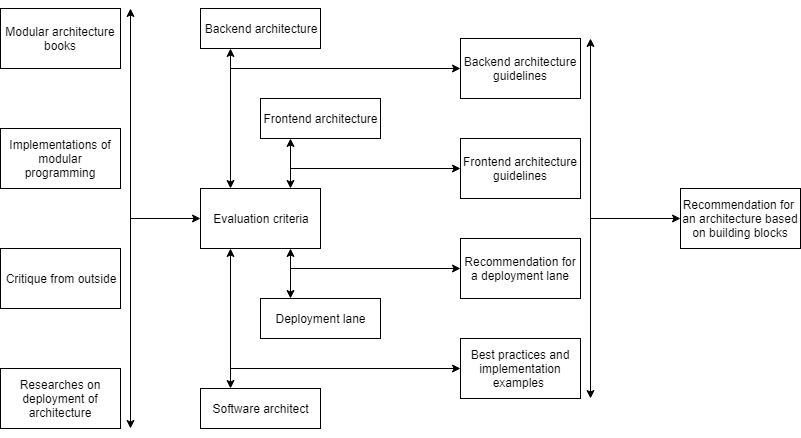
\includegraphics[width=\linewidth]{research_framework.png}
	\caption{Research framework}
\end{figure}

\subsection{Expected Results}

The results will be the guidelines on which the practical part of this research will be based.

\begin{itemize}
	\item \textbf{Backend architecture guidelines: } These are the guidelines on which the backend architecture will be based on. These guidelines will indicate why I choose for a certain approach and what the specific approach is.

	\item \textbf{Frontend architecture guidelines: } These are the guidelines for the frontend. Such as the backend guidelines these guidelines will also contain the reasoning for a certain guideline.

	\item \textbf{Recommendation for a deployment lane: } As mentioned in \fullref{sec:DeploymentLane} the deployment lane can impact the backend architecture and vise versa. This recommendation will be implemented and should thus work perfectly with the backend and frontend.

	\item \textbf{Best practices and implementation examples: } What the project manager experiences and what can go wrong is important to then again pass to the evaluation criteria.
\end{itemize}

\section{Research Questions}
Note: question 2 and 3 will be handled separately for both backend and frontend.

\subsection{Main question}
From this we can derive that the main question is:

\largequote{What is the best way to transform a monolith into a modular architecture, where the services are interchangeable from each other}

\subsection{Question 1}
\label{sec:Question1}
The first question that will be asked is what is the purpose of this question. The first question is about software architecture. How does a software architect create a software architecture. The model can be found in the appendix under Creating a software architecture.

The thicker red lines show the parts of the model I want to explore in the question. Thus the question is:

\largequote{What was the thought process behind choosing certain implementations for the quality attributes of a software architecture?}

This question will explore how a software architect chooses the architecture. This will give more insights into what they consider when choosing an implementations so that their rational can be extracted and taken into consideration.

These are some of the sub questions that will be handled based on this central question
\begin{itemize}
	\item Which techniques are used when mapping the priority and the drawbacks in order to make a decision?
	\item How does the priority of a quality attribute influence the end result or software architecture?
	\item How does the software architect combine the priority, drawbacks and possible implementations to a software architecture?
\end{itemize}

\subsection{Question 2}
\largequote{Which software architectures that focus on modularity are available?}

This question focuses on the architecture that are available. The knowledge of how a software architect chooses the architecture is answered in the previous question \fullref{sec:Question1}. In this question there will be a search on the architectures that are available and how they came to be.. Because of the new perspective gotten from the previous question there can be a more nuanced look at the architecture.

Here are some of the sub questions:
\begin{itemize}
	\item Which are the upsides and downsides of each architecture?
	\item On what level is the documentation and research surrounding the architecture?
	\item Which architecture implements the quality attributes I deemed important best?
\end{itemize}

\subsection{Question 3}
\largequote{Which implementations are there of the solutions provided for modular architecture?}

The solutions or architectures provided from question 2 will have implementations or frameworks. It is important to see which implementation implements a certain choice of the architecture in what way. Other questions that will be answered are:
\begin{itemize}
	\item How mature is the architecture in contrast to the implementations?
	\item How does the language chosen in the implementation reflect to the architecture?
	\item On what level does the framework compromise which is not reflected in the architecture?
	\item How is the community of this implementation?
\end{itemize}

\subsection{Question 4}

\largequote{What are the key elements of in which a software architecture will influence the deployment lane?}

This question hints at the relation between a software architecture and the deployment lane. Right now there is a limited view on how the deployment lane should be and how it can be. In order for the practical research to work there needs to be an answer to these questions:
\begin{itemize}
	\item Which infrastructure fits best with my chosen architecture?
	\item What are the costs of different infrastructures?
	\item How does the infrastructure implement our quality attributes
\end{itemize}


\chapter{Creating an architecture}

This chapter will view what goes into choosing a software architecture. What should you consider when choosing one and why.

\section{What is software architecture}
\label{sec:WhatIsSoftwareArchitecture}

First of all lets define what a software architecture is:

\largequote{Software architecture is the process of converting software characteristics such as flexibility, scalability, feasibility, reusability, and security into a structured solution that meets the technical and the business expectations. \cite{softwareArchitectureDefinition}}

\section{Priorities}

As mentioned in the definition of software architecture \fullref{sec:WhatIsSoftwareArchitecture} a software architecture looks at the characteristics as flexibility, scalability, ect. These characteristics and their sub characteristics are defined by ISO 25010 \cite{iso25010}.

It is important to state the order in which EFFE values these quality attributes. Every decision will be based on this order and will be rationalized by this order.

What is EFFE looking for in an architecture? As mentioned in \fullref{sec:Intention} the first point points out the modularity and the interchangeability of these building blocks. The \textbf{maintainability} quality attribute has reusability and modularity as its sub characteristic. Thus is this the first focus of the software architecture.

The second focus is \textbf{compatability}. Compatibility is the degree to which a product, system or component can exchange information with other products, systems or components, and/or perform its required functions, while sharing the same hardware or software environment \cite{iso25010}. The system can be very modular but if the different functionalities cannot talk with each other you get nothing from the modularity.

As mentioned in first and second point the functionality may be shared between building blocks or not but each building block should be able to be functionality loose from the other building blocks. This is why \textbf{functional sustainability} will be the third focus.

With such a loosely coupled system one issue remains. The \textbf{security}. Because every functionality is loosely coupled it means that the functionalities will talk with each other over an open network or a closed network. If they talk on an open network the security needs to be checked constantly. On a closed network measures need to be taken to keep the network closed. That is the reason on why security is our fourth focus.

After running through these four quality attributes we have an application that can function without being overtaken by unintentional users. But in order to keep the intentional users satisfied the services or functions need to be reliable. Thus \textbf{reliability} will be our fifth focus.

When something is reliable it does not mean it is workable. Because if the site is not responding as fast as possible the user will get irritated and maybe leave the site. A study in 2018 of Google showed that the bounce rate between 3 second load time and 5 second load time is 58\% \cite{bounceRateDifference}. Thus in order for our users to be actually able to use the application in a responsive manner \textbf{performance efficiency} becomes our sixth focus.

There are only two quality attributes left. Portability and usability. Normally there is a good argument about why usability would be higher in the rankings. But because this research more focussed on the architecture of the application and not UX or UI \textbf{portability} will be our seventh focus and \textbf{usability} our eighth.

\subsection{Recap}
\label{sec:IsoRecap}

\begin{enumerate}
        \item maintainability
        \item Compatibility
        \item Functional sustainability
        \item Security
        \item Reliability
        \item Performance
        \item Portability
        \item Usability
\end{enumerate}

\section{What goes into choosing or creating an architecture}

\subsection{Creating an architecture}

So compared to choosing an architecture, creating one is something entirely different. An architecture does not exactly have a creator. This is because an architecture is just blueprint on how to create the software design. This is why the choice was made to interview current software architects and ask them the questions on how they made those choices.

This image was used to show how this research looks at architecture:

\begin{figure}[H]
	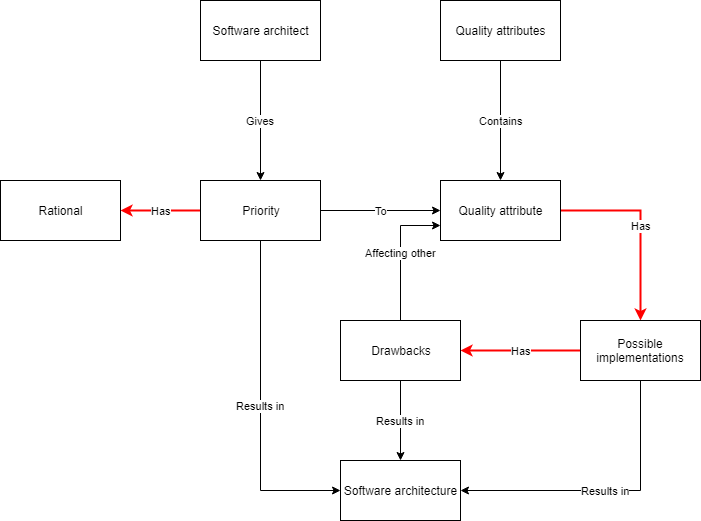
\includegraphics[width=\linewidth]{creating_architecture.png}
	\caption{How a software architecture is chosen}
\end{figure}


\chapter{Modular architecture}
\label{sec:ModularArchitecture}

A modular architecture:
\largequote{Modular design or “modularity in design” is a design approach that subdivides a system into smaller parts called modules or skids that can be independently created and then used in different systems. A modular system is characterized by functional partitioning into discrete scalable and reusable modules, rigorous use of well-defined modular interfaces and making use of industry standards for interfaces. \cite{whatIsModularArchitecture}}

When researching famous architectures in software there are a few examples of non modular architectures. Such an architecture is the layered architecture. In the image below is shown how such an architecture operates.

\begin{figure}[H]
	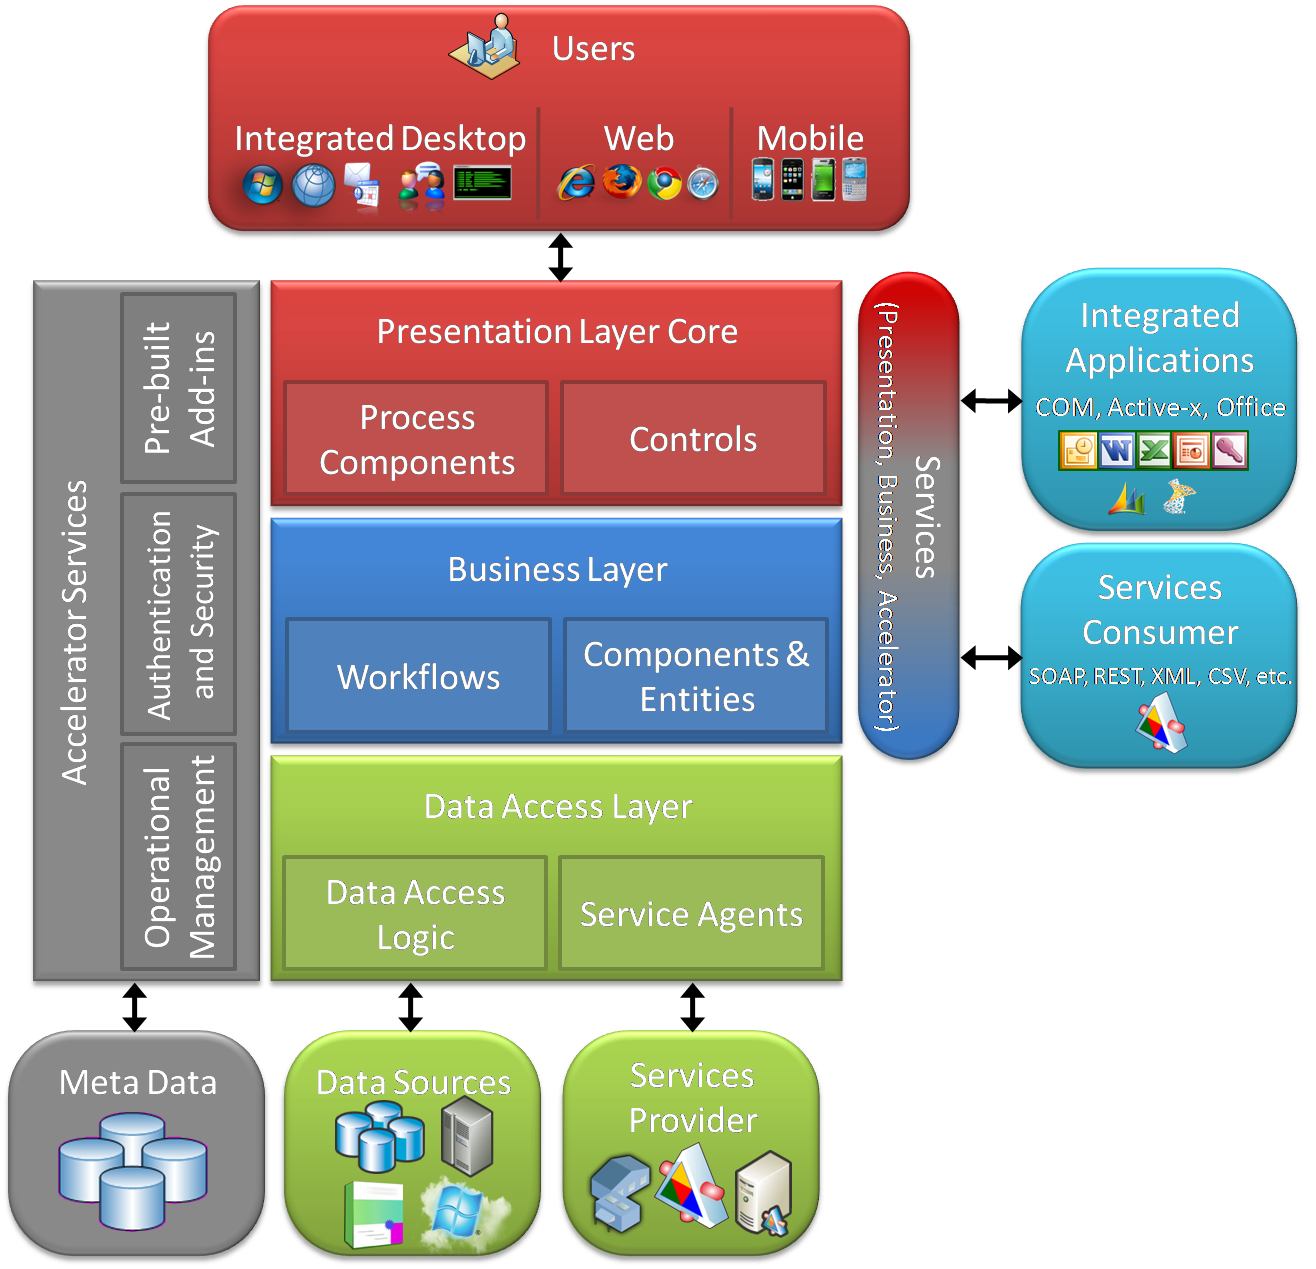
\includegraphics[width=\linewidth]{layered_architecture.png}
	\caption{Layered architecture \cite{layeredArchitecture}}
\end{figure}

As shown in the figure the architecture is layered based on responsibilities. Each layer having its own purpose. The layers can talk with each other but they are intertwined. This means that a class or object in the presentation layer can talk to the same business layer object as another presentation layer class. This concludes in the objects being highly coupled.

A modular architecture is based upon modules. A module is:
\largequote{deployable, manageable, natively reusable, composable, stateless unit of software thatprovides a concise interface to consumers” \cite{moduleDefinition}}

This is eerily similar as the description of what this research calls building blocks in \fullref{sec:TheProblem}

\section{Architectures}
\label{sec:Architectures}

\subsection{Microservices}
If most software engineers in 2019 think of a modular software architecture the first architecture that comes to mind is microservices. In the last years microservices have seen a surge in usage. One of the biggest companies that showed its effectiveness is Netflix \cite{microservicesNetflix}.

\subsubsection{Definition}
The best way to describe a microservice is:
\largequote{A particular way of designing software applications as suites of independently
deployable services. \cite{microservicesDefinition}}

While there is no concrete definition of a microservice there are some characteristics that
every definition contains.
\begin{itemize}
        \item \textbf{Highly maintainable and testable:} enables rapid and frequent development and deployment

        \item \textbf{Loosely coupled with other services:} enables a team to work independently the majority of time on their service(s) without being impacted by changes to other services and without affecting other services

        \item \textbf{Independently deployable:} enables a team to deploy their service without having to coordinate with other teams

        \item \textbf{Capable of being developed by a small team:} essential for high productivity by avoiding the high communication head of large teams \cite{microservicesCharactaristics}
\end{itemize}

Now that there is a clear understanding of what microservices are and which principles
they should follow. Some best practices can be pinpointed.

\subsubsection{Best practices}
The first best practices is to \textbf{create a seperate datastore} for each microservice. First of all not every datastore fits every service. It may be that a message service may achieve more efficiency from a NoSQL database and a user service from an SQL database. A benefit stemming from this is that microservices lets the team think about each datastore used for each service and why that datastore is the correct one for that specific service \cite{microservicesNetflix}.

When creating a separate datastore for each service you run the risk of data inconsistency. For example, there is a user service which stores the user id. There is also a message service which stores the message and the user id to whom the message is send. If a user gets deleted in the user service, this should reflect in the message service. But with microservices this is not automatically the case because each service has its own datastore. Therefore the foreign keys are not native and thus will not be updated or give a warning.

Another best practice is \textbf{writing documentation} \cite{microservicesBestPractice} for each microservice. Most importantly about how they should be used and which interface it uses. For example, when a new service is created next to our messaging and user service called file service which handles the files send in the messages. This service should know how to communicate with the message service. This makes it easier for the new services to connect to the existing services.

Another challenge with microservice is the \textbf{monitoring} \cite{microservicesBestPractice} of the services. Because it is not known how many services are online it is important to know when they are online and what they log. For example, our messaging service is used frequently and duplicates itself. This then means that the logging of the new service needs to be picked up by your monitoring system in order to view the whole picture of the running application.

\subsection{Miniservices}
One of the “new” ones is miniservices. The reason new is between quotes is because most companies that implement microservices actually implement miniservices. The difference between microservices and miniservices is best described in the figure below:

\begin{figure}[H]
	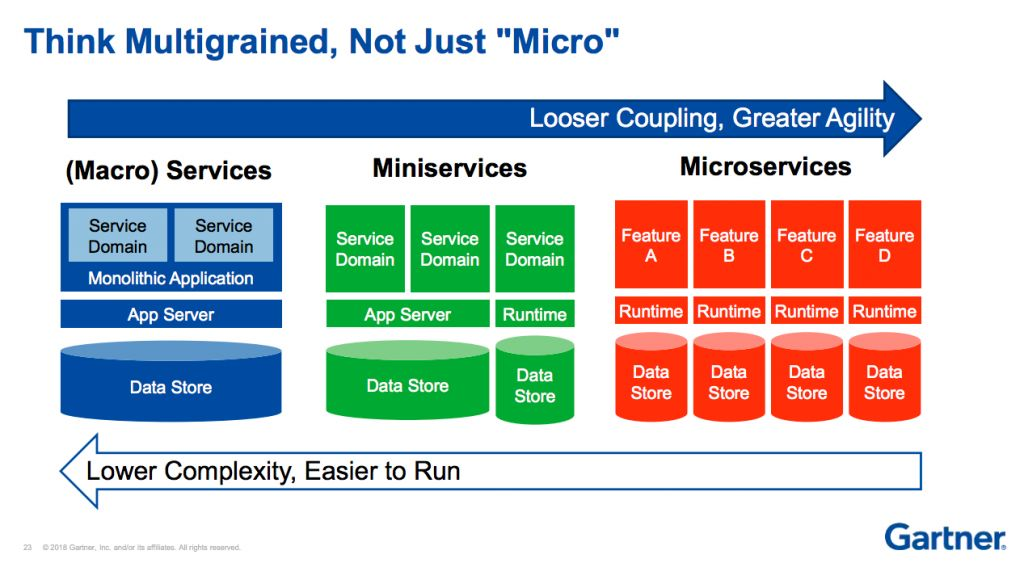
\includegraphics[width=\linewidth]{miniservices.png}
	\caption{Miniservices architecture \cite{miniservicesDefinition}}
\end{figure}

Miniservices is essentially an architecture based on breaking specific rules of microservices \cite{miniservicesOrigin}. As shown in the picture the biggest difference between microservices and miniservices is that microservices are actual features being decoupled and miniservice is about decoupling a domain of features.

This means that each service may contain multiple features but all of the features should be linked to the same domain. Thus the communication inside a service is more fluent and needs less network design than microservices does.

Another divergence is that each microservice should have a separate datastore. This is not the case for miniservices. Every miniservice may be connected with the same datastore \cite{miniservicesDefinition}.

The main advantage miniservices has over microservices is the complexity of the network architecture. With microservices every service is singled out. Which means no service knows about each other so the protocol in which the services speak can be different and may differ from service to service. With miniservices each service connects to the same database. Which makes it easier and faster to do complex querying.

\subsection{Modular monolith}
\label{sec:ModularMonolith}

The main idea behind a modular monolith is preserving the idea of encapsulation but deploying it differently \cite{modularMonolithIdea}. Instead of deploying different services separately with each service having its own datastore, a module can be a library, plugin or namespace. This makes deploying easier to manage whilst still having the modularity gotten from encapsulation.

Just like with miniservices each module will contain the functionalities of a single domain. But unlike the miniservices the modular monolith is compiled to one application instead of multiple.

Modular monolith is perfect for smaller teams because it does not require as much setup as miniservices or microservices.

\section{The comparison}
\label{sec:Comparison}

A good talk about modular monoliths \cite{modularMonolithTalk} shows that most of the time when thinking of architecture there are two extremes. The monoliths and the microservices. As shown in the figure below:
\begin{figure}[H]
	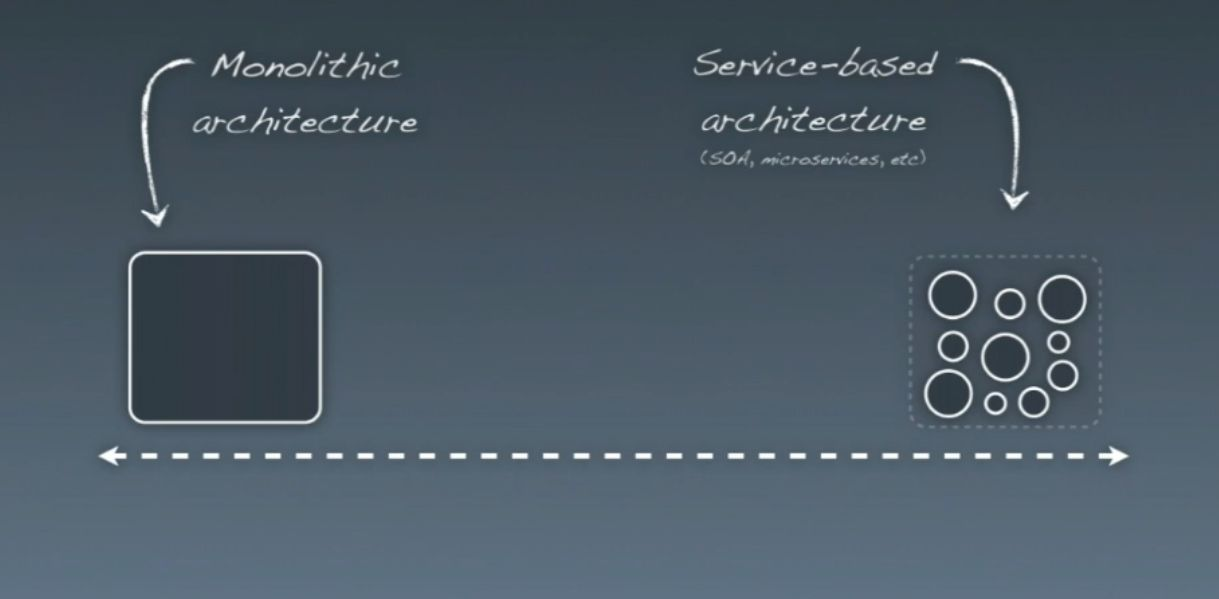
\includegraphics[width=\linewidth]{microservices-spectrum.png}
	\caption{Monolith, microservices spectrum \cite{modularMonolithTalk}}
\end{figure}

But this is not always the case as shown in \fullref{sec:Architectures}.There are cases where microservices are the best choice and there are cases where miniservices or a modular monolith is the best choice. This chapter will further compare the three architectures and decide which architecture fits best with EFFE's priorities. This will be done with the help of chapter \fullref{sec:Priorities}

\section{Complexity}
\label{sec:Complexity}

Complexity always plays a role when choosing the right architecture. Looking at the three architectures shown in \fullref{sec:Architectures} it is obvious that the complexity changes the smaller the modules. Thus the most complex architecture is microservices and the least complex one is modular monolith. With miniservices right in the middle.

In the figure shown below there is an example of the microservice architecture. This shows that each service may have its own datastore but can also run on a different server. This means that each service needs to know in some way where the other services are located. This is called service discovery. Service instances have dynamically assigned network locations. Moreover, the set of service instances changes dynamically because of autoscaling, failures, and upgrades. Consequently, your client code needs to use a more elaborate service discovery mechanism \cite{serviceDiscovery}. This is also the case with miniservices.

\begin{figure}[H]
	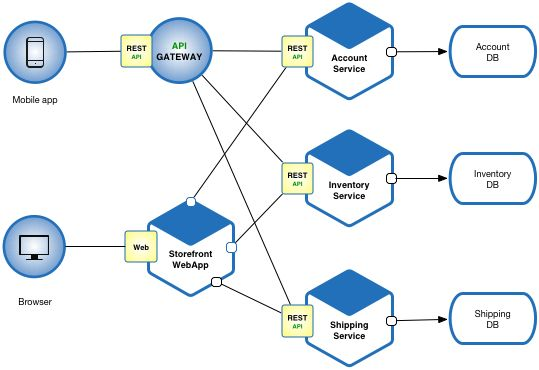
\includegraphics[width=\linewidth]{microservice-architecture.png}
	\caption{Microservice architecture}
\end{figure}

Even though they can connect to a centralized datastore the services do not have any knowledge of each other. In a monolitic application there are no different services. The modules can talk with each other via functions and imports. This means that there is knowledge of the other modules.

The other thing that makes microservices especially complex is the splitted datastores. Because the database is splitted it can be hard to handle foreign keys or pointers to other data objects. This is because the datastore does not have a direct connection to this pointer. This problem of complexity is not prevalent amongst the miniservices and modular monolith because in these architectures the datastore is shared.

The quality attributes that are applicable to this attribute are:
\begin{itemize}
        \item \textbf{Maintainability:} The more complex an infrastructure and/or architecture is the more maintenance it requires.
        \item \textbf{Security:} Complexity always brings security issues with itself. This is especially the case with miniservices and microservices because of the service discovery.
\end{itemize}

\section{Technology}
\label{sec:Technology}

One of the most convincing arguments for choosing microservices is the freedom of choosing the technology. There is a possiblity to write the first service with Node.js and a MongoDB database and the next service with Java and an ElasticSearch datastore. This makes it really easy when switching technology or recruiting new developers.

Miniservices does have the benefit of choosing a different programming language per service. But because all of the services talk with the same datastore, the datastore technology is always the same.

Modular monolith is the worst in this section. A modular monolith is stuck with the same technology for the programming language and the datastore.

The quality attributes that are relevant are:
\begin{itemize}
        \item \textbf{Porability:} The portability is very high because each service can be ported separately which makes it easier.
        \item \textbf{Compatability:} The compatibility between technologies is extremely relevant when looking at the architecture
        \item \textbf{Performance:} Because the technology for each service can be different. A language can be chosen to create the optimal performance for that specific service.
\end{itemize}

\section{Testing}
\label{sec:Testing}

It is known that testing plays a big role in creating reliable software. There are multiple types of testing \cite{testTypes}. Not all of them are useful for EFFE. That is why EFFE has created a list of tests it does on the current application. These are test types that will be looked at:

\begin{itemize}
        \item Unit tests
        \item Integration tests
        \item End-to-end tests
        \item Load tests
\end{itemize}

Each section will begin with a rating from 1 to 3 where 1 is the best architecture for this kind of test.

\subsection{Unit tests}
\label{sec:UnitTests}

\begin{enumerate}
        \item Microservices
        \item Miniservices
        \item Modular monolith
\end{enumerate}

In a microservice each function is its own service. So the functions are really easy to test. Because miniservices is domain based it takes a bit more effort to test the whole service but it is easier than the modular monolith. This is because the modular monolith is more tightly coupled than miniservices.

\subsection{Integration tests}
\label{sec:IntegrationTests}

\begin{enumerate}
        \item Modular monolith
        \item Miniservices
        \item Microservices
\end{enumerate}

Because the modular monolith contains all its services it is easy to test how they work together. This can even be done with unittesting. For the miniservices and microservices it is more difficult. The reasoning behind this is the complexity of the service discovery. To test for example two services, service discovery needs to be setup. Each extra service that is added to the tests will add more complexity. An integration test with microservices may call six different services. But with miniservices it may be less if the functions that are called are in the same domain. This is why microservices is in the last place in this type of testing.

\subsection{End-to-end tests}

\begin{enumerate}
        \item Modular monolith
        \item Miniservices
        \item Microservices
\end{enumerate}

As seen in the \fullref{sec:IntegrationTests} the same type of problem occurs. A function that is called may need multiple microservices or miniservices called.

\subsection{Load tests}

No difference

All of the architectures are equal when it comes to load testing. This is because load testing is done on a live site. This does not mean it has to be done on production, although it can be.

\subsection{Conclusion}

The quality attributes that testing influences are:

\begin{itemize}
        \item \textbf{Maintainability:} Unit testing and integration testing creates an environment that gives the developer a guideline he or she should follow. The developer knows what is expected and thus can maintain the application with more ease.

        \item \textbf{Compatibility:} Almost all of the test types look at if the code works and will fail if it changes. The backwards compatibility Of a application will be tested constantly.

        \item \textbf{Functional sustainability:} This is where testing started. Writing unit tests to be sure the functionality has not changes.

        \item \textbf{Performance:} With load testing performance will be tested this won’t be taken in consideration because there was no difference between the architectures.

        \item \textbf{Usability:} End-to-end testing is specifically made for testing usability. It checks if the UI of an application still behaves the same.
\end{itemize}

\section{Costs}
\label{sec:Costs}

Because EFFE is a startup costs are very important. EFFE does not have the steady money flow that a more mature company may have.

There are two parts on how costs are calculated for software. The first one contains the price of development and the second one is the price of hosting.

Development time and understanding the code go hand in hand. When a developer does not understand the code the developer can not develop. So how do these architectures hold up considering development time and understanding the code?

Microservices as mentioned before is a very complex architecture but when developing it is one of the easiest. Because each function is its own service, creating a service is really easy. There is not a great number of code in one function and therefore easy to understand.

Miniservices and a modular monolith are in the same situation the code can be more complex because they need to talk to other services or modules but there is also a great number of code in one service or module. Therefore understanding the code and the developing time become larger.

The difference between the architectures is not very big. If miniservices and modular monolith are structured in such a way that is logical it should not matter.

Modular monolith is by far the least expensive architecture. Because the application can run on one server without the expense of server discovery it can be run on a server that costs \$5,- a month \cite{digitalOcean}. But the tricky parts comes when talking about interchangeability. What happens if a company wants a building block changed slightly only for them. If they are willing to pay for it it means that there needs to be a whole new server because the application is build on its own. When EFFE has five clients who want this and five clients that run on the standard version. EFFE would have to run it on six servers which would be \$30 dollars on the cheapest server which is not expensive at all.

Microservices and miniservices are the opposite with microservices standing out more. These services require server discovery as mentioned before. There are open source server discovery services such as \href{https://www.consul.io/}{consul} but those also need a seperate server. Server discovery is not the most expensive part. The most expensive part is a combination of having multiple services running on different servers that can autoscale. This means that there is less knowledge about our spendings beforehand.

There are some amazing services that handle deployment and autoscaling for microservices. The most known are Kubernetes, Nomad and Docker swarm. These services however cost \$40,- per month with the minimum requirements. The cost of the servers and the orchestrator can ramp up quickly.

The quality attribute that is most affected by the cost is the \textbf{maintainability}. This is purely because if the infrastructure is this expensive there would be no money to maintain it.

Thus when looking at development time vs infrastructure costs there is a lot to say for the modular monolith. Because even tho the development time is a bit slower for modular monoliths the infrastructure is way cheaper than miniservices or microservices.

\section{Scalability}
\label{sec:Scalability}

It would not be fair to compare these architectures without taking a look at scalability. This is where microservices shine. Microservices are made for horizontal scaling.

Vertical scaling is when hardware resources are added to a server. For example adding 4GB of ram to a server. Horizontal scaling is when adding more instances of the service. This can be on multiple servers \cite{microservicesMultipleServer}.

As mentioned before microservices is created for horizontal scaling. When a service suddenly gets a lot of traffic the service can autoscale itself. This can be done rather easily because the service itself is so small. This is also why it is harder with miniservices and even harder with modular monolith.

Scalability is important when talking about \textbf{performance}. When a server is going above a certain threshold it can duplicate itself and can now split the traffic along the new instance.

\section{Frontend}
\label{sec:FrontendComparison}

When looking at the architecture there is one that stands out as easily adapted for frontend and that is modular monolith. This is because it will still be compiled to one application.

Right now EFFE uses Vue to create a single page application. But this does not mean other frontend frameworks are not considered explained in \fullref{sec:Frontend}.

When looking at microservices in the backend there is a similar phenomenon in the frontend called micro-frontend or micro-apps \cite{microFrontends}. But there is one problem that persists with this solution and that is the sharing of UI elements. There is an option to share them between services but that would mean each service would use the same language and need to be deployed all together if one of those UI elements change. Therefore this is not a solution. A talk about micro-apps (microservices frontend) gave a convincing story about why someone should switch to them \cite{frontendMicroservices}. But when asked about the UI elements there was no answer that fixed this problem.

Concluding that for frontend there is only one possibility for a modular architecture and that is modular monolith.

\section{Recap}

This is a recap of what is discussed in \fullref{sec:ModularArchitecture}. As mentioned in \fullref{sec:Comparison} in this research there will be looked at the quality attributes and how they matched up per architecture.

\fullref{sec:Complexity} talks about the complexity and how it can influence the whole project. The architecture that ended on top was modular monolith and the quality attributes that were applicable where \textbf{maintainability} and \textbf{security}.

In \fullref{sec:Technology} microservices came out on top. With miniservices following and modular monolith as an obvious last. The quality attributes that are influenced by technology are \textbf{compatibility}, \textbf{performance} and \textbf{portability}

\fullref{sec:Testing} was by far the most contested section with no clear winner. But when looking at the types of tests that were considered (unit, integration, end-to-end and load testing) modular monolith ended with the best result with miniservices again in the middle and microservices ending last. The quality attributes for testing are \textbf{maintainability}, \textbf{compatibility}, \textbf{funtional sustiainability}, \textbf{performance} and \textbf{sustainability}

In \fullref{sec:Costs} the clear winner is modular monolith with miniservices following and microservices at an obvious last place. The quality attribute affected by the cost is \textbf{maintainability}

\fullref{sec:Scalability} has microservices at first. In second place is miniservices and last is modular monolith. The quality attribute applicable is \textbf{performance}.

In \fullref{sec:FrontendComparison} there was eventually only one architecture that actually made sense and that was the modular monolith.

\section{Conclusion}

The architecture that fits EFFE best is the modular monolith. The chapters where modular monolith was the best option were also the ones that influenced the quality attribute \textbf{maintainability} the most. As sorted in \fullref{sec:IsoRecap} \textbf{maintainability} is by far the most important quality attribute for EFFE. EFFE also does not have much money as mentioned in \fullref{sec:Costs} Thus costs play a big part in this decision as well. Finally the modular monolith architecture is especially good for small teams and that is a perfect description of the software team of EFFE since it exists out of one person at the moment.

Microservices have the clear distinction of winning the race on technology and scalability but this is not where the focus of this research lays. Although technology aligns with some of EFFE's focusses it does not compete with the main focus that the modular monolith architecture touches on and the pros do not outweigh the cons.

Miniservices is a mixture of modular monolith and microservices and takes some good parts of the both architectures but also some drawbacks of both architectures. The biggest downside is the complexity of the network as explained in \fullref{sec:Complexity}.


\chapter{Implementation of the architecture}

The chosen implementation is modular monolith. As mentioned in \fullref{sec:ModularMonolith} a modular monolith is based on domain driven design where the modules can be developed separately. Most of the principles can be taken from domain driven design. But in a modular monolith the modules do not know what other modules contain. This is possible over an API.

\section{Characteristics}

Domain driven design was coined by Eric Evans in his book Domain driven design \cite{domainDrivenDesign}. Eric Evans himself said that there is no real standard for domain driven design but there is one for a domain:

\largequote{A domain is a field of study that defines a set of common requirements, terminology, and functionality for any software program constructed to solve a problem in the area of computer programming, known as domain engineering. The word domain is also taken as a synonym of application domain It is also seen as a sphere of knowledge \cite{domainDefinition}}

What is important to note is that each module is linked to a domain but there is a distinct difference between only implementing domain driven design and modular monolith. A modular monolith is part of the software architecture of the application while domain driven design part is of the software design. The difference between those two is that software architecture about converting characteristics or quality attributes into a structured solution where as software design is more about the responsibility each module or section, inside the architecture, has. \cite{softwareArchitectureDefinition}

\section{Current situation}

The table below is to paint a good picture of the current application, situation and map which domains there are inside the EFFE application and which functionalities they possess.

\begin{tabularx}{\linewidth}{|>{}X|>{}X|>{}X|}
    \hline

    Domain
     &
    Functionalities
    \\ \hline

    User
     &
    \begin{compactitem}
        \item Reset password
        \item User CRUD*
    \end{compactitem}
    \\ \hline

    Shift
     &
    \begin{compactitem}
        \item Shift overview
        \item Create shift
    \end{compactitem}
    \\ \hline

    Skill
     &
    \begin{compactitem}
        \item Skill CRUD*
    \end{compactitem}
    \\ \hline

    Store
     &
    \begin{compactitem}
        \item Store CRUD*
    \end{compactitem}
    \\ \hline

    Client
     &
    \begin{compactitem}
        \item Client CRUD*
    \end{compactitem}
    \\ \hline

    Authentication
     &
    \begin{compactitem}
        \item Login
        \item Reset password
    \end{compactitem}
    \\ \hline

    Schedule
     &
    \begin{compactitem}
        \item Generate schedule
    \end{compactitem}
    \\ \hline

    Hour registration
     &
    \begin{compactitem}
        \item Hour registration
    \end{compactitem}
    \\ \hline

    Shift market
     &
    \begin{compactitem}
        \item Shift market
    \end{compactitem}
    \\ \hline

    Shift change
     &
    \begin{compactitem}
        \item Switching shifts
        \item Calling in sick
    \end{compactitem}
    \\ \hline

    Company
     &
    \begin{compactitem}
        \item Managing company settings
    \end{compactitem}
    \\ \hline
\end{tabularx}

\small{\textcolor{gray}{* CRUD or Create Read Update Delete refers to the actions that can be called on an object via the rest API}}

An example of a use case where it is needed to replace one of these modules is if a big client comes to EFFE but requests something small that should be different in the user module. With a modular monolith we can create this new module and place it inside the application and it will work the same as the normal application.

\section{API}
\label{sec:API}

When creating this API the assumption is done that a modern ORM(Object relational mapping) is used.

\largequote{Object-relational-mapping is the idea of being able to write queries, as well as much more complicated ones, using the object-oriented paradigm of your preferred programming language. \cite{ormDefinition}}

This assumption is done because almost every modern framework uses this concept to map objects to a relational database which is what EFFE uses.

Therefore the first attribute defined in our api is the \textbf{model} itself.

Microservices talk with each other via a protocol. The most used protocols are HTTP, TCP or AMQP \cite{microservicesAPI}. What all of these protocols have in common is that they return a serialized version of the response. Most of the time in JSON.

Commonly in web frameworks there is something used called a dataclass or a serializer. This class can convert an object into JSON or any other content type. Thus if the api of a module in the modular monolith can expose such a serializer the application can serialize all the foreign keys the module's model has. But when working with the application of EFFE the company found that each user role may require a other specific serializer. For example: EFFE has three roles: the employment agency employee, the client and the temp worker. If the client and the temp worker want to retrieve the shifts the client also gets the users in that shift while the temp worker only sees the general data of the shift. This is so that temp workers won't have the biased in taking shifts with people they like or vise versa.

Therefore it is important to note that each role should have a specific serializer. The API will have \textbf{base serializer} and the option to change the \textbf{serializer by role}.

\section{Programming language and Web framework}

A web framework is:

\largequote{A software tool that provides a way to build and run web applications. As a result, you don’t need to write code on your own and waste time looking for possible miscalculations and bugs. \cite{webFrameworkDefinition}}

It is a industry standard to use web frameworks. It simply makes life easier. But which web framework? The comparison will be of the front- and backend frameworks and languages. There will not be a research of the whole framework or language. The focus of the research will lay on the compatibility of the framework with the modular monolith architecture.

The reason the focus lays on the web framework is because the modularity mostly comes from the framework. Most popular programming languages have the same capabilities when used right. The framework decides how the language is used and also how it reacts to modularity.

\subsection{Backend}
\label{sec:BackendImplementation}

Even though the programming language is important most of the time their modularity comes from the framework that is implemented. According to hackers.io these are the top backend frameworks in 2019 \cite{topFrameworks}

\begin{enumerate}
    \item Express (Node.js)
    \item Django (Python)
    \item Rails (Ruby)
    \item Laravel (PHP)
    \item Spring (Java)
\end{enumerate}

All frameworks will be tested against the same use case:

The first domain is employees. An employee has:
\begin{itemize}
    \item Name
    \item Birth date
    \item Email
\end{itemize}

The second domain is shifts. A shift has four attributes
\begin{itemize}
    \item Title
    \item Start date
    \item End date
    \item Employees
\end{itemize}

The application will provide an api which can do a create, list and retrieve(single object) call for both shifts and employees.

Last of all the modules should only talk with each other via the \fullref{sec:API}.

All of these tests are done using Windows 10 on a Dell XPS 13, using the git bash terminal and the usage of MySQL as the primary database.

The assumption is made that the database exists where \texttt{root} is the username and password. The web framework used is the name of the database table.

All the code can be found at \url{https://github.com/jessielaf/modular_monolith}

Rails and Spring were not successful in the support of creating a modular monolith. Django on the other hand is the only framework that supports this type of architecture out of the box. This already gives the edge to Django as the framework to use. But what amplifies this choice is the amount of code that is needed to write in order for the test to work was minimal in comparison to the other frameworks. Django was also the only framework with build-in database migration generation. This allows the user to create migrations based on the model. This is very important because it eliminates human error when creating migrations by hand.

\subsection{Frontend}
\label{sec:Frontend}

Frontend is a very fast moving lane in software engineering. On october 8th 2010 \cite{angularJs} the first big frontend framework was published called AngularJs. This framework has been maintained by google and received a lot of traction. Three years later at Js ConfUS Jordan Walke of Facebook gave an introduction to React \cite{reactJs}. This changed the frontend world. Mainly because react was not a framework but a library. Which means that you are able to include it in your existing project whereas with Angular you solely have an Angular application. In February 2014 the last big javascript framework would be released called Vue \cite{vueJs}. Vue is often seen as the perfect blend between React and Angular. This is partly because Vue can be used as a library and a framework.

These three frameworks / libraries where chosen because they are the most used and the most loved by the javascript community \cite{allFrontendFrameworks}.

First off there is a need to define what should be in the api of each module in the frameworks. There is only one actual layer the modules should export and that is the service. A service is object which translates the rest api into an object api. They should export all the CRUD functionalities.

The scope of the test is that the frontend application should use our backend site created in \fullref{sec:BackendImplementation}. So the application should be able to do:

\begin{itemize}
    \item Create a employee
    \item List the employees
    \item Detail employee view
    \item List shifts
    \item Add shifts
    \item Detail shift view
\end{itemize}

All the code can be found at \url{https://github.com/jessielaf/modular_monolith}

From the implementations it is obvious that Angular is harder to implement than Vue or React. This is a combination of typescript and dependency injection which Angular uses. Vue and React on the other hand are really similar. But there are a few differences that makes Vue easier to use than React. The first one is the two way binding of Vue \cite{vueTwoWay}. React does not have this feature. What this means is that you have to write your own handler for every different input type. Another difference is that with Vue the router is included. Thus the Vue router is supported by the official team. React does not have a router build in. The best frontend framework for the modular monolith is Vue.

\section{Building the modular monolith}
\label{sec:BuildingModularMonolith}

The application consists of multiple modules and these modules need to be assembled before the application can be used. Assembling the modules should be easy on build when the application is being deployed but also when a developer is cloning the application. The first option is to create a command that will clone all the modules. This can be done per project and with a cli (command line interface) tool or with code inside of the application itself. The best option is the cli because this gives a common interface that can be used in multiple projects. The config for the modules and the projects will look the same. An example of such a system is a dependency managers. Managers such as \href{https://yarnpkg.com/en/}{Yarn} or \href{https://getcomposer.org/}{Composer}. These managers use a JSON file to define which versions are used of which dependencies or in this case modules. The config files for a modular monolith could be more stripped down because the requirements are less when comparing it to a full functional dependency manager.

There are two things all dependency managers have, a \textbf{name} and a \textbf{version}. What is unique to the modular monolith situation is that our name can be the same but where the module is \textbf{located} from can be different. Because there is a possibility that a specific module is required with a different version. This is all module level but there should also some project level settings. Such as the \textbf{directory} where the modules should be copied to.

\begin{verbatim}
    copy_dir: modules
    modules:
      employees:
        repo: git@github.com:jessielaf/employees-module
        version: master
      shifts:
        repo: git@github.com:jessielaf/shifts-module
        version: 1.0
\end{verbatim}

In this example the employees module will be retrieved from git@github.com:jessielaf/employees-module with the latest version and will be copied to \texttt{modules/employees}.

An example how the code could work is below:
\begin{verbatim}
    import yaml
    from git import Repo


    with open("example_config.yml", "r") as stream:
        config = yaml.safe_load(stream)
        modules = config['modules']
        copy_dir = config['copy_dir']

        for name, module in modules.items():
            repo = Repo.clone_from(module['repo'], f"{copy_dir}/{name}")
            repo.git.checkout(module['version'])
\end{verbatim}

Of course this is a very stripped down version of what can be. The best upside to this solution is that it can be the same for frontend and backend. The other option is to add the modules with the use of the framework. This makes it easier to use for new developers because they don't need to install a plugin or dependency that does this. But the code for the frontend and the backend needs to be managed and exists in the repositories. This makes it that the frontend config can be different from the backend one and it creates a harder to understand config. This is why the choice goes to the one config meets all option.

\section{Deployment lane}

As mentioned earlier the architecture that has been chosen for an application can make a big impact on the deployment lane. This is the reason why this section is chosen as an important piece for this research. But the choice of architecture came down to a solution where the deployment lane should not change or only change with building the application as explained in \fullref{sec:BuildingModularMonolith} this can be done with one commando. The deployment lane can thus stay virtually the same as before for EFFE.

\section{Implementing it in the application}

\subsection{Backend}

First of all the module api should be added. This can be done in \texttt{effe/api} and looks like this:
\begin{verbatim}
    from typing import Any
    from dataclasses import dataclass


    @dataclass
    class ModuleAPI:
        model: Any
        serializer: Any
        serializer_per_role: Any = None
\end{verbatim}

The first module that will be converted is shifts. This is because this is the biggest module. If this module can be converted all of them can be. The first thing to do is replace a direct link to the model to a link via the module. This means
\begin{verbatim}
    form shift.model import Shift
\end{verbatim}

Can be replaced with
\begin{verbatim}
    from shift.api import api as shift
\end{verbatim}

The use of the model looked like this:
\begin{verbatim}
    Shift.objects.all()
\end{verbatim}

And can be changed to:
\begin{verbatim}
    shift.model.objects.all()
\end{verbatim}

For the serializers the same principles apply.
\begin{verbatim}
    from shift.serializers.base import BaseSerializer
\end{verbatim}

Can be changed to:
\begin{verbatim}
    from shift.api import api as shift
\end{verbatim}

So when referring to the shift serializer:
\begin{verbatim}
    shifts = BaseSerializer()
\end{verbatim}

To:
\begin{verbatim}
    shifts = shift.serializer()
\end{verbatim}

The first problem that this created is that you cannot import a serializer into a model. This happens because python imports all classes even if it does not use one. Apparently this creates a circular dependency. When python has a circular dependency it gives a \texttt{ImportError: cannot import name} error. There is an open question on stackoverflow that has not been answered yet \cite{circularDependencyQuestion}.

The dependencies of the api need to be lazy loaded. There are two options on how to do this. The first one is to overwrite a function in the api. The ModuleApi would look like:
\begin{verbatim}
    from abc import abstractmethod


    class ModuleAPI:
        @abstractmethod
        def serializer(self):
            pass

        @abstractmethod
        def model(self):
            pass
\end{verbatim}

The api would look like this:
\begin{verbatim}
    from effe.api import ModuleAPI


    class Api(ModuleAPI):
        def serializer():
            from shift.serializers.api.base import BaseSerializer

            return BaseSerializer

        def model():
            from shift.models import Shift

            return Shift

    api = Api()
\end{verbatim}

The other method is string based imports. Where the ModuleApi would look like this:
\begin{verbatim}
    import importlib
    from typing import Dict


    class ModuleAPI:
        _model: str
        _model_package: str
        _serializer: str
        _serializer_per_role: Dict[str, str]

        def __init__(
            self,
            model_package: str,
            model: str,
            serializer: str,
            serializer_per_role: Dict[str, str] = {},
        ):
            self._model = model
            self._model_package = model_package
            self._serializer = serializer
            self._serializer_per_role = serializer_per_role

        def model(self):
            return getattr(importlib.import_module(self._model_package), self._model)

        def serializer(self):
            return importlib.import_module(self._serializer).BaseSerializer
\end{verbatim}

And the api:
\begin{verbatim}
    from effe.api import ModuleAPI

    api = ModuleAPI("shift.models", "Shift", "shift.serializers.base")
\end{verbatim}

The first options is better. This is because the model is imported directly this means that when renaming models or paths some IDE's will pick it up themselves. It is also more explicit and pylinters will pick up if a module cannot be imported.

Switching to the new api was easy until the user shift view needed to be changed. This view shows the the shifts of one user and the shift change requests of a user. This means that inside the shift serializer the shift change request serializer should be applied. But to make sure there are no circular dependencies this can't be done inside the \texttt{BaseSerializer} of the shift module. So there needs to be a function on which fields need to be serialized. Thus the api needs to be rewritten.

The django rest framework uses a private field \texttt{\_declared\_fields} that contains the nested serializers. The new api looks like this:
\begin{verbatim}
    from abc import abstractmethod
    from typing import Dict

    from rest_framework.serializers import Serializer


    class ModuleAPI:
        @abstractmethod
        def _serializer(self):
            pass

        @abstractmethod
        def model(self):
            pass

        def serializer(self, serializers: Dict[str, Serializer] = None):
            base_serializer = self._serializer()

            if serializers:
                for name, serializer in serializers.items():
                    base_serializer._declared_fields[name] = serializer
                    base_serializer.Meta.fields.append(name)

            return base_serializer
\end{verbatim}

In the shift overview the field shiftchangerequest\_set should be serialized by the shift change request serializer. The serializer looked like this:
\begin{verbatim}
    serializer_class = serializers.ShiftOverviewSerializer
\end{verbatim}

And with the modular monolith looks like this:
\begin{verbatim}
    serializer_class = Shift.serializer(
        {
            "shift_change_request": ShiftChange.serializer()(
                read_only=True, source="shiftchangerequest_set", many=True
            )
        }
    )
\end{verbatim}

The class \texttt{serializers.ShiftOverviewSerializer} can be removed because it is not used anywhere anymore.

In order to use the cli described in \fullref{sec:BuildingModularMonolith} cleaner, a project was made. It can be found at \url{https://github.com/jessielaf/modad}.

To implement this there needs to be a creation of the config in \texttt{modad.yml} which looks like this:
\begin{verbatim}
    dest: .
    modules:
        - name: shift
          repo: git@github.com:jessielaf/effe-shift
          version: master
\end{verbatim}

Then push the shift module to github at \url{https://github.com/jessielaf/effe-shift}. And remove the shift module from the base application and add shift to the .gitignore so github does not push the module to the base applications git. Now this command can be ran
\begin{verbatim}
    modad assemble
\end{verbatim}

Now the shift module is pulled from the github repository and in the application.

\subsection{Frontend}

The first module that was implemented in the backend was the shifts module. But EFFE uses Nuxt.js as a framework on top of Vue. Nuxt creates the routing via the folder structure. But this folder structure is decoupled from the business logic. There are two options to fix this:

\begin{itemize}
    \item \textbf{Adding two directories}: The API as described in \fullref{sec:API} needs to be changed so it will also handle multiple directories where it should copy to.
    \item \textbf{Rewriting it to only Vue}: As shown in \fullref{sec:Frontend} Vue is capable of having a modular monolith architecture. But to get this there needs to be a rewrite of the whole frontend application. There is a lot that can be refactored but there are also a lot of Nuxt.js functionalities the application uses.
\end{itemize}

Even though the second option ties more into the modular monolith architecture, the first option is better for a proof of concept for EFFE.

The config in \texttt{modad.yml} is needed to initialize our modular monolith is:
\begin{verbatim}
    dest:
        - src: pages
          dest: pages
        - src: module
          dest: modules
    modules:
        - name: shift
          repo: git@github.com:jessielaf/effe-ui-shift

\end{verbatim}

This will clone the most of the code into the \texttt{src/modules} and pages into \texttt{src/pages}. This is a one way street. The modules will now only be cloned. But by this logic the modules can also be created from this config. This makes it easy to use in development. Just load a module, change somethings and pull it back up. Thus the assembler also needs to dissemble the modules. This dissembler looks at the config and based on it, it creates a new folder with the changes made to the directories that are copied by the assembler.

The current shift module is intertwined with the change request, availability and shift market modules. The first action is to remove these from the shift module. Next up is the api for the shift module. Because Nuxt.js is used instead of only Vue the api looks a bit different:
\begin{verbatim}
    export default class Api {
        static create(axios, object, options = {}) {
            console.log(object, "not saved");
            console.error("Implement the create functionality");
        }

        static update(axios, id, object, options = {}) {
            console.log(object, "not saved");
            console.error("Implement the create functionality");
        }

        static retrieve(axios, id, options = {}) {
            console.log(id, "not retrieved");
            console.error("Implement the retrieve functionality");
        }

        static overview(axios, options = {}) {
            console.error("Implement the overview functionality");
        }
    }
\end{verbatim}

The same command as in the backend can be ran here:
\begin{verbatim}
    modad assemble
\end{verbatim}

The application works as it did before.


% \chapter{Deployment Lane}

The deployment of a project means making the project available to reach with needed minimal setup. The most common one is running a web application. The minimal setup is running a web browser. This is also how the modular monolith will be deployed.

Almost all of the websites you visit will be hosted on a server. A server is a computer which is open to the public on specific ports. This means that the server can serve a website on port 80(http) for example. What can diver is where the server is hosted and maintained. This can be on SaaS services like \href{https://www.heroku.com/home}{Heroku} which manages the server as well as maintaining it and setting it up. The other option is something like \href{https://www.digitalocean.com/}{DigitalOcean} or \href{https://aws.amazon.com/}{Amazon web services}. These companies manage the server but do not set them up. The big difference is you can run multiple instances of a web app on one server. Also you have complete access of the server which may be very important if you want to secure certain bits of your application. The last option is an on premise server. This means that you own the physical server and have it at your office. The big risk is if the server crashes or brakes your whole company will be down. The best option is obviously the usage of services like Digital Ocean and Amazon web services. Which one you use is not important for this research but how we use them is.

\section{Operating system}

The first thing to consider is the operating system. There are two big players when it comes to the operating systems of servers. Windows and Linux. While linux is not a operating system in and of itself it is the ground layer of a lot of other famous operating systems such as ubuntu and debian. The reason linux is often considered better for a server are \cite{linuxBetterThanWindows}:
\begin{itemize}
  \item Free and open source
  \item Stability and Reliability
  \item Security
  \item Flexibility
  \item Hardware Support
  \item Total Cost of Ownership (TCO) and Maintenance
\end{itemize}

So what is the best linux distro? It really comes down to preference \cite{bestLinuxDistro}. Right now EFFE uses Debian in production. That is why this is the choice of linux distro.

\section{Setting up servers}

In order to setup a server you can go into the command line and type all the commands yourself until it works. This is of course very easy when you are only deploying one application but when you want a scalable infrastructure this becomes harder and harder. So what you need is a service that sets up the server.

Right now EFFE uses \href{https://www.ansible.com/}{Ansible}. What makes ansible so great is that is can be run on your own computer. Some other options require one dedicated server that handles the configuration of all the servers. This means that the infrastructure gets bigger and bigger. That may be important to a bigger company but EFFE wants its server configuration to be handled easily but with version control. Another alternative to Ansible is \href{http://www.fabfile.org/}{Fabric}. This is a python library that allows you to run commands on a server.

There are other options. The most well known are \href{https://www.saltstack.com/}{SaltStack}, \href{https://puppet.com/}{Puppet} and \href{https://www.chef.io/}{Chef} but all of these solutions require a master server. This is something EFFE does not want as explained in the previous chapter.

There are two differences between ansible and fabric. The first one is pretty obvious when using both. Fabric uses python to write your configuration and ansible uses yaml. Ansible is written in python but the yaml is what you write. Base on the yaml files ansible decides what to run when. The other big difference is that ansible has preconfigured modules. This means that if you want to, for example, install a package you don't write the whole command, as with fabric, but you define the module and the packages. To get a clear understanding an example is shown below:

Fabric:
\begin{verbatim}
  connection.run('sudo apt-get install python3 python3-pip')
\end{verbatim}

Ansible:
\begin{verbatim}
  - apt:
      pkg:
        - python3
        - python3-pip
\end{verbatim}

A byproduct of this is that the output handling is way better with Ansible. This is why Ansible is the choice for our use case.

\section{Deploying}
Deploying is a different story. Ansible is just to setup the server but when deploying you preferably want to do that based on the activity of your project. There are a few services that allow this. Once again it is important that this software does not add another server to our infrastructure. Possible solutions are:
\begin{itemize}
  \item \href{https://about.gitlab.com/}{Gitlab} has a free tier with 2,000 pipeline minutes per group per month \cite{gitlabFreeTier}
  \item \href{https://buddy.works/}{Buddy} offers a free tier where 120 executions per month with maximum of 5 projects \cite{buddyFreeTier}
  \item \href{https://circleci.com/}{CircleCI} offers a free tier with 1,000 build minutes per month \cite{circleCIFreeTier}
  \item \href{https://codefresh.io/}{Codefresh} has a free tier with no constraints on build minutes or executions \cite{codefreshFreeTier}
\end{itemize}

When looking at these services codefresh stands out because it does not have build time or project limitations. Therefor this is the service we will use for deployment.


\chapter{Conclusion}

After the introduction the research ranks the quality attributes. This is done in order to find which architecture fits best with EFFE's needs. The architectures that were considered, were modular monolith, miniservices and microservices. These architectures have in common that their main focus is modularity. The rankings of the architectures is:
\begin{enumerate}
  \item Modular monolith
  \item Miniservices
  \item Microservices
\end{enumerate}

The modular monolith is ranked first, because focusses on modularity while still being able to be developed by a small team with limited resources. Which is amplified when looking at complexity and costs. This is where the modular monolith architecture excelled. Because in the end the modular monolith is compiled to one application, the complexity is a lot lower than the other options. Lower complexity leads to lower costs. The service discovery together with an orchestrater can already ramp up the costs and modular monolith does not dependent on either one.

The best backend framework for the modular monolith is Django. This is because Django, by design, already implements domain driven design. A modular monolith decouples it modules by domain. So a framework that has such a functionality built in already has an advantage. The other feature of Django, that Rails, Spring, Express and Laravel did not have out of the box, was migration generation. This feature makes it easy for the developer to create migrations without human error that may be involved.

For the frontend Vue was the best framework. Both Vue and React were easy to implement the modular monolith in, but Vue has two way binding out of the box. In React there was a need to write these two way bindings for every different input. Angular uses dependency injection. In order to make this work smoothly with the api of the modular monolith a great number of code had to be written per module.

To build these modular monoliths a new project was created called modad. This is a modular monolith assembler and dissembler. It uses a yml file as config to create the modular monolith and load its modules on build time. The choice to create a new project instead of implementing it in the codebase was made because modad can be used for backend and frontend. While if it was implemented in the codebase the frontend and backend assembler would look different and that adds complexity.


\chapter{Sources}

\printbibliography[heading=none]


\chapter{Appendix}

\section{Interviews}
\subsection{Questions}

In order for the interview to go smoothly it is important to define the questions beforehand. The questions will be based on the research framework and the evaluation criteria. The interviews will be conducted by Jessie Liauw A Fong and the interviewee will be a software architect.

Questions about how they view software architecture:
\begin{itemize}
  \item What is software architecture?
  \item What is your company the main job of a software architect?
  \item Which with kind of architectures have you worked?
  \item What is the biggest pitfall when implementing a new architecture?
  \item How do you decide which architecture is best of a certain project?
  \item What is the architecture that you implement in most of your projects? (Frontend and backend)
\end{itemize}

Questions about how they view modularity:
\begin{itemize}
  \item What is the first thing that you think of when I say modular architecture?
  \item What are the most upcoming architectures that are focused on modularity in your opinion?
  \item Which programming languages do you think compliments a modular architecture best?
  \item
\end{itemize}

Questions about the chosen architecture and method:
\begin{itemize}
  \item What do you think of the image about how I went my way in choosing the right architecture?
  \item What is your opinion about domain driven design
  \item Have you ever heard of modular monolith
\end{itemize}

\begin{figure}[H]
	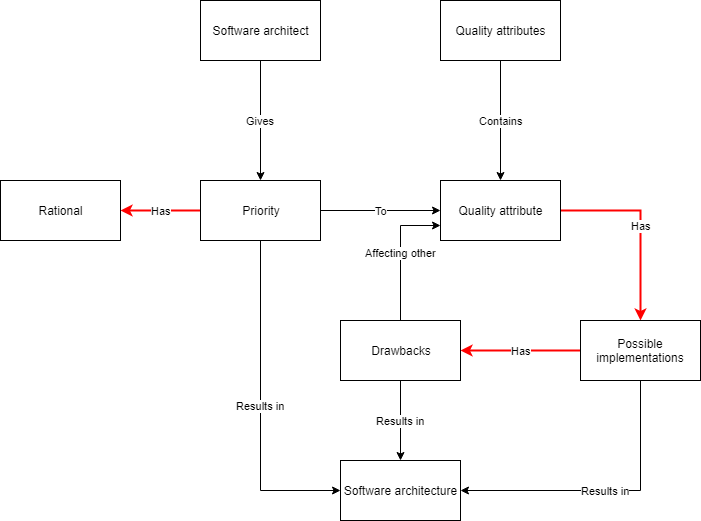
\includegraphics[width=\linewidth]{creating_architecture.png}
	\caption{How a software architecture is chosen}
\end{figure}

\subsection{Interview with Joris}
\subsection{Interview with Joris}

Jessie: Na mijn eerste vraag aan jou is eigenlijk. Wat is in jouw ogen software architectuur?

Joris: Nou dan hadden weer meteen ook. Heb je een half uurtje?

Jessie: Als je het zo beknopt mogelijk zou moeten uitleggen aan iemand.

Joris: Dan is het sofware architectuur een model van hoe een stuk software geimplementeerd is. Het is een soort abstractie. Als je kijkt naar de architectuur van de auto bijvoorbeeld, de motor bestuur en de deur. Op dat niveau zo kun je ook de software kijken. Software verdeel je ook op een bepaalde manier in min of meer onafhankelijke delen en die delen hebben vervolgens de relatie met elkaar. Dus aan het stuur draai gaan de wielen zo. Als ik software dit hier gebeurt, gebeurt er ergens anders iets anders. En architectuur een van de definitie van architectuur is een soort gedeeld model, gedeeld met engineers en de eigenaar van de software. Over hoe die software nou opgedeeld in brokken en hoe die brokken gezamenlijk werken om de functionaliteit geimplementeerd te krijgen.

Jessie: Ja.

Joris: Korter dan dat krijg ik het niet.

Jessie: Nee dat is een goeie beschrijving. En binnen Ximedes, hebben jullie daar iemand die echt alleen op de software architectuur zit?

Joris: Nee, bij ons is er, vrijwel elk team rol van software architect. Typisch, tegelijkertijd ook de meest ervaren developer. Dus bij ons is de architect ook, die bouwt mee. Meestal wordt er op een bepaald niveau wel iets gedocumenteerd over de architectuur. Met name voor mensen die niet in het team zitten dus opdrachtgevers of mensen die nieuw komen. Ik denk dat in de meeste gevallen de architectuur nog veel meer een gedeeld begrip is binnen zo'n team of dat nou echt een los product is. We hebben ook niemand die alleen maar architect is en niet bouwt.

Jessie: Hoe documentaireserie die architectuur?

Joris: Ja dat wisselt. Ook dat wij werken voor verschillende opdrachtgevers die ook zelf verschillende mensen en eisen hebben. De meeste projecten hebben een document, word document bij wijze van spreken of markdown. Vrije teksten en daar wordt in opgeschreven wat mensen. Het is een beetje een soort cirkel definitie maar daar schrijven op wat het team nodig vindt om op te schrijven.

Jessie: Ja.

Joris: Dat dat wisselt heel erg voor detailniveau. Wat ik altijd deed, ik heb zelf ook gearchitect. Je beschrijft het systeem als geheel met de grove delen is sommige. Sommige stukken ga je even de diepte in. Omdat er bijvoorbeeld iets interessants gebeurt if iets niet voor de hand liggend. Want 9 van de 10 keer zeker bij ons geval wij schrijven code van, typisch project van 40000 regels of zo dus dat moet je. Als je naar kijkt moet je toch wel. Het idee is dat we zulke code schrijven dat als je er naar kijkt je het toch wel snapt. Dus dan hoef je niet helemaal te gaan zitten documenteren.

Jessie: Ja.

Joris: Maar goed daar naast zijn er best een aantal klanten vroeger meer dan nu. Die het heel formeel gedocumenteerd willen hebben. Dingen als uml unified modeling language. We deden het al niet veel en we doen het nu nog minder, omdat klanten het niet meer nodig vinden.

Jessie: En als je dan kijkt naar de verschillen architecturen die binnen Ximedes worden gebruikt. Eelke zijn dat en waarom is daar voor gekozen?

Joris: Ja. Ik denk met afstand de meest voorkomende architectuur is een monoliet. Java of tegenwoordig kotlin, maar een web applicaite op JVM. Die communiceert met relationele databases. En dat of een server sided gerenderde html ui heeft of rich client zoals react, angular of vue die communiceert via de rest api. Ik denk dat dat 80 procent van de projecten zijn. En dat kiezen we omdat we, we geloven er heel erg dat je dingen zo eenvoudig mogelijk moet maken. En dat is een kunst, daar zijn geen harde regels voor maar door de bank genomen is een monoliet voor developers, voor beheerders, voor eigenaars. Eenvoudiger dan een microservices architectuur bijvoorbeeld. En dus als je kijkt naar microservices als alternatief van een monoliet. Dat is nogal wat investeringen die inkomt. Het wordt complex op te bouwen, complex om te deployen. Het lost een hele specifieke set aan problemen op die lang niet elk klant heeft. Voor de de de lood en de performance en de security die wij nodig hebben is een monoliet uitstekend. Dus dat is een beetje de defacto standaard. En wat je vervolgens ziet is dat je per project per klant daarin wordt afgeweken daar waar het nodig is en daar waar het zinnig is. Dus soms worden systemen in 2 delen op in 3 delen of 20 delen opgesplitst.

Jessie: Je wilt je kijkt gewoon naar bijvoorbeeld. Als er 1 deel is wat eigenlijk 9 procent van de loadopvang dan wil je eigenlijk alleen deel onderscheiden.

Joris: Ja, bijvoorbeeld.

Jessie: Dat je die makkelijker kan delen en dat de rest van de applicatie in een instance kan draaien.

Joris: Ja bijvoorbeeld, security is bijvoorbeeld een ander ding. Waarbij je zo min mogelijk footprint service er naar buiten wil laten zien. En 9 van de 10 keer zijn de klanten. Voor developers is er niks handigers dan gewoon een proces wat ik kan starten met dat gedoe en zit je ook weer met je git repositories. Kijk alles schaalt. We hadden ook een project draaien. Die is gestart en die had op een gegeven moment 20 git repositories en die jongens werden dood ziek. Die hebben het nu allemaal in een monorepo gestopt. Dus we zijn continu opzoek.

Jessie: Ja precies ja.

Joris: Kijk en als je facebook bent is het een ander verhaal. Dan heb je een heel team zitten die de hele dag niks anders doet dat repositories managen. Ja zijn we met een mannetje of 4/5 per team zo gaat het.

Jessie: Ja dat snap ik. Oké en als ik het goed heb begrepen hebben jullie wel microservices of hebben jullie wel andere architectuur geïmplementeerd binnen het bedrijf? Wat was de grootste challenge die pitfall die je zag tijdens het implementeren waar je die eigenlijk pas daarna dacht ik van oh ja oké als we dat eerder hadden gedaan. Was het een stuk makkelijker geweest. Of is het vooral tijd dat gewoon?

Joris: Kijk als we even teruggaan naar architectuur als mentaal model van hoe de software werkt. Los even van hoe het deployed wordt, meer aan de binnenkant. Ik kan niet zeggen dat als bedrijf er nou wel of niet iets geleerd is, maar ik heb wel software gebouwd waarvan ik achteraf de dacht. Een goed voorbeeld ik heb ooit software gebouwd voor een lease bedrijf, ING Lease. En dat automatiseerde het verkopen traject. Zo'n lease contract bestaat uit onderdelen, het is een beetje als een hypotheek, je hebt garantor en zekerheden noem het maar op. Complexe gedoe pricing dingen en dat aan de eind van de rit moesten er documenten komen. In het nadenken in het ontwerpen van het systeem. Hebben we heel lang gepraat over dat sales process. En die documentatie was een soort afterthought, oh ja aan de eind van de rit moeten het documenten worden. Ik denk dat letterlijk 3/4 jaar later toen het systeem al heel succesvol was toen merkte we opeens. Toen bleek dus dat er heel veel changes kwamen op die documenten en dat veel mensen ontevreden waren en achteraf. Hadden we met veel meer vooruit die document generatie moeten behandelen. En nu is het een systeem wat contract workflow automatiseerd en achteraf een document maakt. We hadden het als een document generator moeten bouwen die ook wat contractmanagemend deed. Dat is zo'n architectuur dingen waar je later bijna niet meer vanaf komt. Tenzij je het compleet herbouwd. Dat gezegd hebbende. We proberen hier tijdens een project gaat tijdens de bouw heel erg op te letten. Bijna agressief te refactoren als we merken dat het niet meer klopt. Uiteindelijk begin je op een gegeven moment maar te bouwen en dan ga je een kant op, dan heb je een model. En tijdens de bouw merk je. Daarom is het zo fijn dat je snel naar klanten teruggaat, omdat die klant komt met dit bedoelde ik niet. Soms blijkt gewoon dat je een verkeerd zit je domeinmodel. Ja dan los je dat op.

Jessie: Is wat je eigenlijk zegt is dat. En wat je hebt geleerd dat je gewoon eerst gaan kijken van oké wat wat is nou echt het meest grote gedeelte of tenminste de meest belangrijke functionaliteit die de applicatie daadwerkelijk heeft. Waar draait het allemaal om en daar ga je omheen bouwen in plaats van eerst het bouwen, bepalen wat je wilt bouwen en waar je eigenlijk naartoe wilt gaan.

Joris: Hier geloven we sowieso heel erg  ook als wij agile werken. Dan nog beginnen altijd met noem het workshops. Gesprekken met de klant, eerste proof conceptcode. Om een beetje te spelen met de oplossingsrichtingen en daar van tevoren over na te denken. En dat gekoppeld met ijdens de bouw vrij agressief refactoren als je merkt dat het niet goed komt en niet op z'n loop laten gaan dan wordt het een puinhoop. Maar de realiteit is dat je het gewoon ook niet altijd kan voorspellen. We hebben software die soms 10 jaar misschien nog wel langer in productie draait. De wereld veranderd ook in 10 jaar. De software wordt gebruikt voor toepassingen waar ze in 't begin nooit voor bedacht zijn. Dus al heb je het helemaal goed in het begin. De kans dat het over 5 jaar nog matched met waar dan voor gebruikt is, is heel klein. Hoe dan ook is het geen statisch ding. Continu de oplossing vinden bij de realiteit van het bouwen.

Jessie: Dan hebben we het stukje echt over de software architectuur gehad. Nu ga ik wat vragen stellen over modulariteit binne de architectuur. En eigenlijk het eerste wat ik je wat vragen is: waar denk jij aan als ik als ik het heb over een modulaire architectuur.

Joris: Modulair impliceert natuurlijk min of meer ontkoppelde onderdelen, modules. Dus als je zegt modaire architectuur dan verwacht ik dat je het hebt over hoe die bestaat uit onderdelen waarbij het voor sommige onderdelen misschien ook wel meer dan 1 implementatie is. Die dus optioneel zijn. Die je wel of niet hebt. Dat je misschien wel twee of drie versies van dezelfde module hebt. Die je min of meer als een soort legoblokjes inelkaar klikt. Nu vul ik heel veel in op basis van het woord modulair.

Jessie: Dus dat is goed. En als je kijkt naar de modulaire architectuurs die bestaan in de industrie. Welke denk jij zegmaar dat de meeste potentie heeft en daarbuiten ook goed implementeerbaar is als dat een beetje duidelijk vraag is.

Joris: De vraag is wel duidelijk. Ik weet alleen niet of ik er wat zinnigs over zeggen. Kijk dat had ook te maken met mijn achtergrond. Wij bouwen maatwerk software in opdracht waarbij we elke keer met een wit vel beginnen en zelden hoeven rekening gehouden met het feit dat dezelfde software bij het meer dan een klanten draait bijvoorbeeld. Waarbij dus ook zelden de noodzaak is om echt dingen plugable te maken. Dus in die zin heb ik er niet heel veel ervaring mee. Ik weet wel dat voor ons de paar keer dat we hebben geprobeerd dit te doet het altijd erg tegenviel. Moeilijk is om het goed te doen. En goed nogmaals voor ons de return on investment er bijna nooit was om dat in de praktijk werd module a nooit vervangen door module b. Ik heb wel eens nagedacht over plugins enzo. Het lijkt me verschrikkelijk moeilijk om in een keer goed te doen. We hebben wel een beetje ver van weet want we doen het eigenlijk nooit.

Jessie: Ja en als je kijkt naar de, dit is veel meer low level. Als je kijkt naar de programmeer talen. Welke programmeer taal denk je dat het beste modulariteit complementeerd, modulaire architectuur. Als je denkt aan die plugins.

Joris: Ik zou in ieder geval naar een statisch getypte taal gaan. Dus Java, C\#, Kotlin noem het allemaal maar op, maar niet javascript, want je wilt wel echt. Ik 1 van de dingen die je natuurlij heel strak moet hebben in een oplossing is het interface. Is het contract tussen 2 modules.

Jessie: Ja.

Joris: Een deel van dat contract zijn je types. Welke berichten gaan erover en wat zit erin, wat is optioneel, wat is een string, wat zijn de validaties op die string. Als je kijkt naar code, als je dat contract wilt uitdrukken in code. En dan zou ik helemaal gek worden als ik daar geen getypte taal gebruik. Het alternatief is natuurlijk dat je interfaces gaan over het netwerk gaan. Het is dan altijd REST of SOAP of van die dingen. Dan maakt de taal natuurlijk weer minder uit. Binnen de getypte talen zou ik niet 1 2 3 een soort voorkeur hebben dat de ene taal geschikter voor dit soort architectuur dan andere.

Jessie: Misschien ook framework specifiek?

Joris: Ja ik denk dat je meer richting de frameworks gaan. Zeker aan de javascript kant. Dingen als spring

Jessie: KTor?

Joris: Ja KTor. Dat gezegd kotlin kent ondertussen wel contracten. Contracten gaat nog een stap verder dan types bijvoorbeeld een onderdeel van wat je tegenwoordig in kotlin kan uitdrukken. Als je deze functie aanroept, dan komt er altijd een positief integer uit. En dat gaat verder dan zeggen een integer. Ja want want er is geen type in kotlin die positieve integers typed dus je hebt meer nodig dan alleen maar de types dus daar zou je nog naar kunnen kijken maar dan praat je heel erg over sdk level. En ik denk eerlijk gezegd dat het hangt van je van je project af. Als jij een plugin structuur hebt waarbij je bij runnende code, code injecteert. Ja ,dan heb je het over dit soort dingen. Als je het hebt over modules die via het netwerk communiceren dan maakt het eigenlijk niet uit.

Jessie: Dat is natuurlijk ook een van de krachten van microservices, dat je niet overal dezelfde taal hoeft te gebruiken.

Joris: Ja, exact. Dat je polyglot kan zijn. Dat je het aan de verschillende teams over kan laten.

Jessie: Dat was het stukje over modulariteit. Ik heb zeg maar een architectuur gekozen. En ik heb daarr deze eigenlijk een soort van flow diagram bij gebruikt. De Rode lijnen heb ik onderzocht. Wat ik eigenlijk heb gezegd is een software architect geeft prioriteiten aan een quality attribute. Die quality attributes zijn door ISO 25010 gedefinieerd. Die quality attributes hebben mogelijke implementaties. Al die implementaties hebben mogelijke drawbacks. En uiteindelijk doormiddel van je prioriteit te koppelen met die drawbacks kom je uit op een software architectuur. Mist er iets in dit plaatje of zeg je als ik een software architectuur kies kijk ik er anders naar.

Joris: Ja, dit is wel aardig bedacht. Ik denk zelden in dit soort formele termen, maar kijk waar ik het wel heel erg mee eens ben is dat architectuur een afweging is tussen verschillende belangen die die onder spanning staan. Security performance begrijpelijke code noem maar op.

Jessie: Allemaal dingen die je uit de ISO 25010 komen.

Joris: Ja die hebben het ook vaker gedaan. Kijk een andere definitie van architectuur zou het zou zeker kunnen zij precies dit. Een gewogen afweging van wat we voor een stuk software wat prioriteit geven en waar we dus de pijlen laten vallen. Dus als je zegt ik ga 100\% voor performance. De kans dat je leesbare code krijgt is de lager en andersom ook. Dus in die zin vind ik het een mooi plaatje. Alleen het zegt meer over het proces van hoe kom ik op een architectuur dan de architectuur zelf, maar dit klinkt heel redelijk.

Jessie: Dan is mijn volgende vraag, ik neem aan dat je weet wat domain driven design is?

Joris: Ja

Jessie: Wat zijn jouw gedachtes erover? En hoe, als je dat implementeerd. Hoe implementeer je dat binnen Ximedes?

Joris: Ja hoe heet die man ook alweer? Erik Evans? Ik heb ooit een boek gelezen en ook een workshop van hem gehad. Dus ik vind dat ik vind de ideeën heel interessant en ik denk ook dat er. Ik had het een tijd geleden over die workshops die we altijd doen. Hoewel we bij Ximedes nooit dus echt domain driven design volgens het boekje hebben gedaan. Merk je wel dat, een belangrijke uitkomst van zo'n workshop is inderdaad zo'n gedeeld domeinmodel. Gedeeld besef van hoe een subset van de wereld werkt. Neem mijn lease software van daarnet. Dat is een complex ding, met contract, pricing, scenario en dat soort dingen. Een goed deel van die workshops simpelweg bedoeld om developers te laten snappen hoe die businees werkt. En ook een beetje om die business te laten verslappen wat de beperkingen van de implementatie van software. Als dat zo doen kun je dit wel, maar dat lukt niet. Dat vind ik wel echt heel mooi. Wat wat we naar mijn weten nooit gedaan hebben. Is dit zo formeel als Erik Evens het bedoeld doorgetrokken naar de implementatie? Wat ik een interessant idee vindt van hem is dat je zegt van ja, dat mag. Dus zoals ik het me nog herinner, tijd geleden, kom ik tot het domein model en dat komt 1 op 1 terug in de software en is ook 1 op 1 hoe je requirements uitdrukt. Ja ik vind het een prachtig idee, heel formeel. Wij doen het niet. Ik heb het ook nooit gedaan dat. Ook hier zie je met al dat soort dingen zal d'r een.

Jessie: Het is een heel groot verschil tussen tussen theorie en implementatie?

Joris: Nou ja en d'r zitten voor een redelijke mate van compleetheid in. Ik snap ook in het boek natuurlijk een soort extreme maar in de realiteit ga je nooit helemaal naar dat punt want het de return on investment wordt steeds lager, maar ik denk dat we dat als Erik Evans naar onze workshop zou kijken dat hij wel redelijk tevreden was. Als je naar de code kijkt een stuk minder. Een consequentie van domain driven design helemaal doorvoeren naar de implementatie is dus dat je ook al die bounded context dingen en dat dat is wel heel. Onze software is gewoon simpeler. Wij vallen toch heel vaak terug op. Ik heb objecten en ik heb value objecten dus objecten waardes in zitten. Ik heb een service laag waar ik methodes op kan aanroepen. Dat we dan weer documenteren en ik heb wat lijm tussen die dat allemaal aan elkaar zet. Dat is geen domain driven design maar het werkt wel lekker.

Jessie: Als ik me goed kan herinneren heb ik aan jullie eigenlijk 2 implementaties. Eentje was eigenlijl layered architecture, maar jullie deden ook wel iets, ook domain driven design. Dat je 1 package had die over een domain ging.

Joris: Ja. Ja we hadden met name 1 architect. Die is weg, maar goed dat heeft hier niks mee te maken. Ja ik heb daar heb ik altijd wel mee geworsteld. Ook dat vind ik het heel idee. Alle software die ik bouw is altijd gelayered.

Jessie: Ja ja, precies

Joris: Waar ik altijd naartoe neig. Vervolgens als je het 1, 2 keer abstracte trekt. Heeft het te maken met die keuze. Java software maar ik denk elke software in de wereld valt in eerste orde uiteen in een aantal noemen het packages, noem het, maakt me niet zoveel uit wat je kiest. En wat je altijd ziet. Wat je ook kiest. Daar zullen altijd concerns zijn. Quality attributes in jouw plaatje. Die daar dan vervolgens niet lekker in passen. Als ik een layard architectuur maak. Dan is een gegeven stuk functionaliteit vanuit een use case verdwijnt opeens door allerlei verschillende plekken en allerlei verschillende lagen. Als ik zeg mijn primaire modules zijn mijn use cases. Dan vallen andere dingen weer een beetje in het niet. Bijvoorbeeld de database logica zit dan ineens op allerlei plekken tegelijkertijd. Hoewel ik het. Ik vond het een heel interessante dat een keer wat anders dan dan dan klassieke three tier layered. Maar het zal ook hier weer per project. Ook hier moet je weer een keuze maken. Eigenlijk heb hier ook weer architectuur te pakken. Hoe je dat een gegeven project een gegeven klant gestructureerd. Het hangt ervan af. Ja, het is ook dat je je hebt ook heel erg hebt te maken met de verwachting van een engineer die over 5 jaar op je project zit. Ik kan natuurlijk heel wild gaan en zeggen ik ga het allemaal anders doen vandaag. Maar dan optimaliseer je niet voor die arme ziel die opeens bugs moeten gaan zitten fixen. Dat zit ik ook wel heel erg mee. Het zijn lastige dingen.

Jessie: En? Heb je wel eens gehoord van een modulaire monoliet.

Joris: De term hoor ik vandaag voor eerst.

Jessie: Oké dus. Snel uitgelegd. Het is eigenlijk domain driven design. Dus je hebt eigenlijk verschillende lagen en dat zijn allemaal domains. Die praten met elkaar over dezelfde api. Bijvoorbeeld:  User of employee heeft een shift. Dan heeft een shift een many to may relation met een employee. En die many to many relationship wordt gedefinieerd via het interface van employee. Employee heeft een interface en daarom weet shift welk moedle hij moet gebruiken. Elke module dus die exporteert ook altijd maar 1 model. En zo heb je eigenlijk de toevoeging dat elke module kan in een aparte repositories worden gedeveloped, door aparte teams. En die kunnen on build time bij elkaar komen. Snal je een beetje wat ik bedoel?

Joris: Ja, maar jouw voorbeeld als ik een shift module maak. Ik moet wel een concept van employee kennen. Is dat mijn eigen implementatie of moet ik op compile time de employee module kennen?

Jessie: Het kan op compile time. Als je niet als je niet met een compiled taal gebruikt.

Joris: Ja precies, ik moet wel het employee concept kennen?

Jessie: Ja klopt, je kent het employee concept. Hetzelfde als dat eigenlijk microservices werken. Je moet weten dat er een andere microservice is die een bepaalde actie ondersteund, maar het interface of de rest api is hetzelfde als bij andere microservices. In plaats dat je een interface hebt over de daadwerkelijke rest api of graphql of whatever. Heb je het nu over de code. Hoe je praat over de code. Een voorbeeld in spring is dus bijvoorbeeld als je dus verschillende layers hebt dat je dan een nieuwe jpa object implementeerd en dat je daarin meteen kan zeggen api.employees is de foreign key. Dus het model wat gekoppeld wordt. Dat is dus wat ik heb gekozen en ik wou je eigenlijk vragen: Wat is je eerste reactie hierop als je dit hoort? Als het nog niet duidelijk heb ik ook een code voorbeeld.

Joris: Het is half duidelijk, maar los daarvan. Mijn vraag is eigenlijk welk probleem los je op? Het klinkt complex en meer werk dan alles gewoon in een monoliet gooien. Dus waarom doe je dit?

Jessie: We omdat het idee is dus als jij. We hebben 1 basis applicatie en laat zeggen er een hele grote klant naar ons toe, maar die wilt 1 module anders hebben. Dan kunnen we nu zeggen oké we bij switchen die modellen switchen gewoon om. Want dat is nu mogelijk omdat je dus omdat ze sowieso over dezelfde api praten kan je ook gewoon een hele module eruit halen kun je de nieuwe module erin stoppen. De applicatie werkt vanzelf nog steeds het zelfde.

Joris: Maar de beperkingen zitten in je api. Daar zitten je grenzen van je vrijheid.

Jessie: Misschien ook wel weer een. Omdat die is maar 1 model mag, leveren eigenlijk. Het geeft wel weer een soort van. Je moet er wel weer meer nadenken over de architectuur voordat je eigenlijk zo'n module begint. Je moet deze wel geaccepteerd worden. Als er maar 1 model wat wat dit model gebruikt moet het dan wel een hele eigen module worden, ect, ect. Dat zijn eigenlijk de afwegingen ervan.

Joris: Ja precies.

Jessie: Dat is eigenlijk waar ik ben gekomen. Dus als je dit even snel hoort wat zijn je eerste reacties? Hoe denk jij erover?

Joris: Nou ik denk dat je over de goeie dingen druk maakt. Als je zegt, laten we zeggen dat wij meegaan met je uitgangspunt die modulariteit nodig is. Daar heb ik geen mening over. Als het nodig is dan maak je, je over de goeie dingen druk. Ja ik weet te weinig van het domein om een verdere mening of dit wel slimmer is dan iets anders, maar het klinkt wel heel redelijk. Wat ieder geval klopt naar mijn gevoel is dat je zegt. Je maakt planning software toch? Daar gaat het om. Kijk linksom of rechtsom. Nou je zou nog een case kunnen maken. Beperk je nou niet teveel tot de plannen van de employees. Maar dat zijn precies het soort ideeën natuurlijk waar je over moet nadenken. Kijk software die alles kan kun je niet verkopen want die doet niks. Dus je moet een soort toepassing hebben. En daarbinnen weer zoveel mogelijk verschillende klanten kunnen bedienen zonder dat je allerlei if statements moet doen. Ja, dat vind ik heel goed en ik vind het een interessant idee om dit pluggability mogelijkheid te combineren met een soort domain driven design analyse. Waar lopen mijn entiteiten nou. Dat vind ik eigenlijk wel heel slim ik heb daar nooit of zo. Ik heb die 2 dingen nooit gecombineerd in mijn hoofd.

Jessie: Dat is dus het onderwerp van mijn scriptie.

Joris: Ja dat je een heel goed onderwerp te pakken hebt. Ja leuk. Goed idee.

Jessie: Dat was eigenlijk dat waren eigenlijk al mijn vragen. Dankje wel voor het interview

Joris: Ja graag gedaan. Niks leukers dan lullen over het vak.

Jessie: Dat vind ik dus ook.




\end{document}
